% Copyright (c) 2008-2009 solvethis
% Copyright (c) 2010-2016,2018 Casper Ti. Vector
% Public domain.
%
% 使用前请先仔细阅读 pkuthss 和 biblatex-caspervector 的文档,
% 特别是其中的 FAQ 部分和用红色强调的部分。
% 两者可在终端/命令提示符中用
%   texdoc pkuthss
%   texdoc biblatex-caspervector
% 调出。

% 采用了自定义的(包括大小写不同于原文件的)字体文件名,
% 并改动 ctex.cfg 等配置文件的用户请自行加入 nofonts 选项;
% 其它用户不用加入 nofonts 选项,加入之后反而会产生错误。
\documentclass[UTF8]{pkuthss}
% 如果的确须要使脚注按页编号的话,可以去掉后面 footmisc 包的注释。
% 注意:在启用此设定的情况下,可能要多编译一次以产生正确的脚注编号。
%\usepackage[perpage]{footmisc}

% 使用 biblatex 排版参考文献,并规定其格式(详见 biblatex-caspervector 的文档)。
% 这里按照西文文献在前,中文文献在后排序(“sorting = ecnyt”);
% 若须按照中文文献在前,西文文献在后排序,请设置“sorting = cenyt”;
% 若须按照引用顺序排序,请设置“sorting = none”。
% 若须在排序中实现更复杂的需求,请参考 biblatex-caspervector 的文档。
\usepackage[backend = biber, style = caspervector, utf8, sorting = none]{biblatex}
\usepackage{amsmath}
\usepackage{graphicx}
\usepackage{booktabs}
\usepackage{pgfplots}
\usepackage{caption}
\usepackage{subcaption}

% 对于 linespread 值的计算过程有兴趣的同学可以参考 pkuthss.cls。
\renewcommand*{\bibfont}{\zihao{5}\linespread{1.27}\selectfont}
% 按学校要求设定参考文献列表的段间距。
\setlength{\bibitemsep}{3bp}

% 设定文档的基本信息。
\pkuthssinfo{
	cthesisname = {本科生毕业论文}, ethesisname = {Doctor Thesis},
	ctitle = {论文图片中定位行内公式}, etitle = {Find Inline Formulae in Pictures of Theses},
	cauthor = {张浩然},
	eauthor = {Zhang Haoran},
	studentid = {1500010684},
	date = {2019年6月},
	school = {数学科学院},
	cmajor = {信息科学系}, emajor = {Some Major},
	direction = {深度学习},
	cmentor = {马尽文教授}, ementor = {Prof.\ Somebody},
	ckeywords = {神经网络,公式检测}, ekeywords = {First, Second}
}
% 载入参考文献数据库(注意不要省略“.bib”)。
\addbibresource{ref.bib}

\begin{document}
	% 以下为正文之前的部分,默认不进行章节编号。
	\frontmatter
	% 此后到下一 \pagestyle 命令之前不排版页眉或页脚。
	\pagestyle{empty}
	% 自动生成封面。
	\maketitle

	% 此后到下一 \pagestyle 命令之前正常排版页眉和页脚。
	\cleardoublepage
	\pagestyle{plain}
	% 重置页码计数器,用大写罗马数字排版此部分页码。
	\setcounter{page}{0}
	\pagenumbering{Roman}
	% 中西文摘要。
	% Copyright (c) 2014,2016 Casper Ti. Vector
% Public domain.

\begin{cabstract}
	公式是我们在论文中比较关心的对象,而行间公式在很显著的位置,行内公式则不容易快速分辨。将论文图片中的行内公式快速定位并识别,是一件有意义的事情。若把这看作一个目标检测的问题,则可以使用经典的目标检测算法去解决这个问题。又或者以这个问题的特殊性为基础,先做图像预处理,进行单词分割,再使用分类器对单词图片进行分类,选出公式图片。这篇文章使用了一系列基础的图像处理手段并用神经网络作为分类器,参考了一些复杂的模型来提高性能。
\end{cabstract}

\begin{eabstract}
	Test of the English abstract.
\end{eabstract}

% vim:ts=4:sw=4

	% 自动生成目录。
	\tableofcontents

	% 以下为正文部分,默认要进行章节编号。
	\mainmatter
	% 各章节。
	\include{chap/chap1}
	% Copyright (c) 2014,2016 Casper Ti. Vector
% Public domain.

\chapter{具体实现}

\section{数据处理}

\subsection{tex文件到图片}
\noindent

我们首先从网上获得了大量的论文tex文件。tex语法中行内公式有明确的标注,通过正则表达式找到其中被\$...\$框住的公式部分,由于我们的关注点只在于行内公式,故被\$\$...\$\$框住的行间公式部分需要排除,找到后在公式外加上可以框住公式的LaTeX命令,并分为使用红框和使用白框两个版本。使用白框的是我们进行训练的主要数据,红框版本是获得标记使用的。为了支持我们新增的LaTeX命令,仍需要使用正则表达式检测是否含有我们需要的宏包,若没有则在开头加上。接着将处理完毕的tex文件编译为pdf文件,在编译过程中发现大量的编译失败,主要原因一是使用的tex文件较为久远,主要为2001-2003年的数据,编译格式和使用的宏包各种各样或已淘汰,缺少相应的宏包支持,二是有的文件的编码格式不是utf-8,而编译时统一以utf-8为标准,故导致了读取失败。成功编译的pdf中也有少量缺失正文,只有公式存在。而且由于为了迅速编译,故所有文件只进行了一次编译,这样所有的参考文献引用都不会生效,参考文献的编号都变成了?,认为不影响本工作,所以忽略该问题。

然后是将pdf文件转化为png图片。由于预计使用工具magick来进行转化,而为了全程使用python编程,故使用了magick的python包PythonMagick,而此包缺少文档说明,故一开始转化为png时遇到了困难,故使用的是jpg格式,这样输出的图片数据大小比较大。在查阅了许多解决方法后才终于得到了png文件,发现相同尺寸下png格式的图片只有jpg格式的几分之一,大大减小了硬盘占用,加快了数据传输。

以上方法都写在了文件texf\_topng.py中。宏包使用了re, os, pdflatex, PythonMagick, PyPDF2, 并导入了自己写的图片处理工具文件。re为使用正则表达式的宏包,pdflatex是将tex编译为pdf的宏包,PythonMagick是将pdf转化为png的宏包,PyPDF2是辅助pdf分页生成图片的宏包。在生成图片的同时裁去了图片的空白边框并通过生成的图片是否有红框来删去了不带公式的图片,以减少不必要的数据。单个tex文件处理使用文件ttp.py,批量文件处理使用ttpb.py。通过以上方法生成了红框版本和白框版本共计16万张图片,每张图片的生成速度在一秒以内,实际生成时使用并行处理。本方法由于还要将论文图片分割为单词,故实际使用的图片数没有这么多。

\subsection{单词分割及数据预处理}
\noindent

单词分割主要分为两个部分,文行分割与行内单词分割。以下处理均使用灰度图像。行和是指图像矩阵一行中非空白元素的比例,由于提前做了图像反转,白色为0,黑色非零,故只需要将一行二值化后求和除以列数,故称为行和。文行的中心行和指文行中间一行的行和,同理,开始行和和结尾行和指文行开始行和结尾行的行和。

在处理之前首先判断图片方向,认为一般只有正向和逆时针90度方向。由于灰度图像白色为255,黑色为0,故先将图片矩阵反转为白色为0,黑色为255,再分别求得图片矩阵的行和和列和。如果图象是正向的,空白边框也已经被截去,故认为行和中0的比例应大于列和中0的比例,因文行和文行之间有固定的空白,而单词与单词之间的空白位置每行不一。以此作为是否要将图片旋转的依据。此判断只对整页论文有效果,若进行单行或单个单词测试则无效,故设置为可以关闭。

文行分割这个问题上,文行与文行之间有明显的空行,以空行作为文行的边界即可。由于只关心行内公式,故文行分割还有更多的要求,需要在分割时排除行间公式和一些特殊的文行,如一条直线、图表、页码、特殊符号等。故以空行作为边界分割后,又以中心行和,前四分之一行和,开始行和,结尾行和和行高度作为标准来去掉不符合需求的文行。行间公式和一条直线这种情况,一般高度与正常的文行有差别,行间公式大部分高度比较大,一条直线、特殊符号等则是高度比较小,故筛选出高度在平均高度一定范围内的文行。而页码则是中心行和极小,实际上行间公式的中心行和也小于正常文行的中心行和。同时行间公式的前面通常是一片空白,故同时使用前四分之一中心行和来同时作为辅助标准。开始行和和结尾行和则是为了去掉图表。在文行分割上如果出现更多的特殊情况还需要更多的标准,这里只写出了我实际遇到的问题。

文行分割后,就是对每一文行进行单词分割了,我们使用的都是英文文档,故这里只考虑英文的单词分割。同样预先进行图像反转,使得白色为0,黑色非零。单词分割与文行分割有相似之处,同样是利用单词与单词之间的空白。但容易注意到一行内的空白有三种情况,单词与单词间的空白、字母与字母间的空白和另外一些比较大的空白,如一行结尾后还有大片空白,每段开始文行的开头空白等。这些空白的位置使用列和就可以轻易找到,接下来就是在这些空白中筛选出单词间空白。由于最后是利用空白的位置来分割出单词,故认为大片空白和单词间空白是同一性质。这里使用的是最小二乘法,找到使得公式最小的空白宽度,然后认为在这宽度以上的都是用来分割单词的空白。这样做的效果还不错,大多数单词都可以分割出来,少数情况下会出现一个单词被分为两个,而常见的情况是一个长公式被分割为多个单词。

以上单词分割不仅可以分割出单词图片,同时可以获得分割出的文行的位置和每个文行中每个单词的位置,结合去除空白边框时获得的左上角的非空白元素的位置,可以将每个单词的位置精确地还原。

将白框版本的图片进行了单词分割,获得了单词图片及其位置,在通过其位置信息在红框版本的图片中检查该单词是否被红框框住,以此获得每个单词的标注。这样我们将原本的图片整理成了单词图片、单词位置信息和单词标注信息,训练神经网络只需要单词图片和标注信息,故将这部分做成tfrecords文件以备后续使用。由于一张论文图片中非公式单词比公式单词要多得多,故这里采用了过采样,将公式图片直接复数拷贝,使得公式图片与非公式图片的数量接近。过采样后实际使用的单词图片为100万张左右。

\section{网络结构与算法}

\subsection{激活函数与损失函数}
\noindent

神经网络中有两个重要的部分,一个是激活函数,一个是损失函数。激活函数是实现网络非线性化的重要手段,常用的激活函数有sigmoid函数、tanh函数和ReLu函数等。其中sigmoid函数和tanh函数由于当输入比较大时会有梯度接近0的问题,即梯度消失,使得非监督训练的效果较差。ReLu函数如下:
$$relu(x) = 
\begin{cases} 
0& x < 0\\
x& x \ge 0
\end{cases}$$
ReLu有计算简单迅速而且不会有梯度消失问题的优势。ReLu仍有些问题,一是若训练发散,会迅速增大或减少到nan,使得结果报错。故开始训练前应仔细检查网络的设置,确保能够收敛。二是ReLu函数将小于零的值直接变为0,使得该输出都为正值,故可能会造成某些神经元的失活,不管怎样训练都为0。同时ReLu的输出都为正值,使得收敛比较困难。故针对ReLu有许多的改进的函数。Leaky ReLu函数为在ReLu的基础上,在$x<0$时加上一个较小的斜率。PReLu则是使得这个斜率作为一个可以训练的参数加入网络中,RReLu的做法则是将这个斜率根据均匀分布随机抽取。PReLu的输出更近接近0,收敛速度比ReLu更快,故我使用的是PReLu。

分类问题使用的最普遍的的损失函数是交叉熵函数$$- \sum_x p(x) \log q(x)$$ 要使用交叉熵函数需要输出和目标都满足概率分布,故交叉熵函数一般结合softmax函数$$softmax(y)_i = y'_i = \frac{e^{y_i}}{\sum^n_{j=1} e^{y_j}}$$将输出和目标都归一化。在二分类时也可以使用sigmoid函数$$sigmoid(y) = \frac 1 {1 + e^{-y}}$$将输出转化为$[0, 1]$之间作为概率使用。在二分类时,softmax的表达式为$$softmax(y)_1 = \frac{e^{y_1}}{e^{y_1} + e^{y_2}} = \frac 1 {1 + e^{y_2 - y_1}}$$ 故神经网络输出的两个值的差与只输出一个值是等价的,差别在于前者的全连接层会有更多的训练参数。我实际使用的是sigmoid函数。

\subsection{神经网络优化算法}

\subsubsection{指数衰减学习率}
\noindent

神经网络的学习率代表神经网络参数的更新速度,较大的学习率使得参数每次更新的幅度较大,收敛得更快,但可能会导致无法收敛到最小,每次更新的时候都跳过了能够收敛到最小值的范围;学习率太小又会导致参数更新太慢,网络收敛速度太小。一般而言,开始时希望学习率比较大,使得网络快速收敛,然后学习率逐渐降低,使得收敛更为准确。故使用了如下阶梯状指数衰减学习率,将学习率乘上一个指数衰减率,使得学习率随着训练次数逐渐降低。实际为每学习1000轮将学习率乘以0.9。

\subsubsection{批标准化batch normalization}
\noindent

神经网络中的数据在经过每层的处理后数据分布可能会发生变化,这一过程被称为Internal Covariate Shift\cite{bn}。这种数据分布的变化传递到后层网络中,后层网络也需要不停地去适应这种分布的变化,这就导致了网络的收敛速度下降。如果采用的是饱和激活函数,如sigmoid或tanh,数据分布变化会导致数据变大进入梯度饱和。而如果是ReLu激活函数,则会有数据分布差异大,深层网络收敛困难的问题\cite{bn-relu}。

由于以上问题,我们使用了batch normalization方法,即对每层的数据做规范化。对一层中的一批数据的每个通道$\{x_i : 0 \le i \le n\}$,做如下规范化操作
$$\mu = \frac 1 n \sum^n_{i = 1} x_i$$
$$\sigma^2 = \frac 1 n \sum^n_{i=1}(x_i - \mu)^2$$
$$\hat{x}_i = \frac{x_i - \mu}{\sqrt{\sigma^2 + \epsilon}}$$
$\epsilon$是为了防止方差为0。这样规范化后每一层网络的数据分布都变得稳定,但数据的表达能力却缺失了。为了获得原有信息,BN又引进了两个可以在网络中进行学习的参数$\gamma$和$\beta$,使得规范化后的数据可以通过变换$\tilde{x}_i = \gamma \hat{x}_i + \beta$恢复表达能力。当$\gamma^2 = \sigma^2, \beta = \mu$时,$\tilde{x}_i = x_i$,即是完全恢复为原来的数据。这样我们既使得每层的分布变得稳定,又能够保证数据的表达能力。规范化是在一个batch的每个通道上做,而偏置项对于一个通道而言是相同的,故只需要对卷积输出做规范化,然后加上偏置项就可以了。

BN使得网络的每层数据的分布变得稳定,后层网络不必去适应输入的变化,实现了每层的独立学习,提高了整个网络的学习速度。在使用ReLu激活函数时,由于ReLu函数的输出都非负,故输出平均值远离0,网络不容易收敛,若不使用BN,使用MSRA初始化30层以上的网络也难以收敛\cite{bn-relu}。同时BN处理后,将降低网络中的参数的敏感度,使得调参,如初始化、学习率等的设置更为容易,不用担心参数的变化随着网络层数加深被放大。使用BN后,也不用担心数据经过多层网络后落入饱和性激活函数的梯度包和区,从而可以缓解使用sigmoid,tanh等激活函数的梯度消失问题。同时BN并没有完全保留原始数据的信息,而是通过学习参数$\gamma, \beta$来一定程度上保留数据的表达能力,这就相当于给数据加入了随机噪音,可以起到正则化的效果,防止数据的过拟合。在原作者的结果中,BN可以在没有dropout的情况下同样达到很好的泛化效果,而且网络的收敛速度提高了很多。\cite{bn}我在网络中也同样使用了BN。

\subsubsection{滑动平均}
\noindent

滑动平均,或指数加权平均是一个使得神经网络模型在测试数据上更加健壮(robust)的方法,在计算网络输出时,使用的网络模型不是当时的模型,而与一段时间内的历史模型有关。变量$v_t$在更新为$t$时刻的取值$\theta_t$时,使用公式
$$v_t = \beta v_{t-1} + (1 - \beta) \theta_t$$
上式中$\beta \in [0, 1)$,$\beta$一般取值较大,即变量在更新时使用了上一时刻的取值,做了某种平均,这样不需要保存一段时间内的每个网络就可以获得某种网络的均值。在网络训练的后期,网络会在在一定范围内波动,使用滑动平均后的网络变量来测试数据就能提高测试结果的表现和稳定性。注意到在网络训练的前期我们希望模型可以更新得更快,故希望衰减率较小,来使得变量快速学习更新。Tensorflow提供了tf. train. ExponentialmovingAverage函数来实现滑动平均,还提供了参数num\_updates来实现动态设置衰减率的大小,使得网络前期衰减率较小,可以快速学习更新,训练到一定程度后则使用较大的衰减率来实现更好的滑动平均。

\subsubsection{过拟合优化}
\noindent

大规模的神经网络有一个重要的难题存在,那就是容易过拟合。神经网络在学习中容易过度学习训练数据的特征,将数据中的噪音也一起学习下来,从而在测试集上的表现效果和训练集上差异较大。

处理过拟合有许多的方法,其中上述的BN就能在一定程度上取得效果。另外一个常用的方法是正则化。正则化是在损失函数后加上一个刻画模型复杂度的函数。
$$J(\theta) = J_0(\theta) + \lambda R(w)$$
$\theta$代表神经网络中所有要学习的参数,$w$表示网络权重,$J_0(\theta)$代表原损失函数,$R(w)$使用中对网络复杂程度的刻画,$\lambda$为模型复杂损失在总损失中的比例。再使用优化算法,如梯度下降时,不是直接优化$J_0(\theta)$,而是同时优化$R(w)$,为的是减小模型的复杂程度,使得模型没法刻画全部的数据信息。若网络的权重值较小,即使输入增大一些,输出也不会变化太多。而若权重值较大,输入的较小变化也会被放大。

常用的正则化有$L1$正则化和$L2$正则化。$L1$正则化的公式为
$$R(w) = ||w||_1 = \sum_i|w_i|$$
$L2$正则化正则化公式为
$$R(w) = ||w||_2^2 = \sum_i|w_i^2|$$
$L1$正则化和$L2$正则化都能够缓解过拟合,不同之处在于$L1$正则化会让参数变得稀疏,即许多地方为0。这是因为$L1$正则化为方形,有许多突出的棱角,这些棱角容易成为优化的结果,而这些棱角上的取值是稀疏的。$L2$正则化则是平滑的,不会使得参数变得稀疏,而且$L2$正则化是可导的,优化更简单。实践中常常同时使用$L1$和$L2$正则化。我只使用了$L2$正则化。

除了正则化,另一个常用的防止过拟合的优化方法是dropout。\cite{dropout}dropout形式简单,就是以一定概率使得神经元失活,即输出为0,dropout在防止过拟合问题上的效果非常好。为了解决过拟合问题,会想到训练多个模型做组合取平均等,这样就需要大量时间去训练模型。而dropout以一定概率使神经元失活,就相当于取了网络的子网络,如果是有n个节点的神经网络,每个节点以50\%的概率失活,则相当于$2^n$个网络的集合,而要训练的参数却是不变的,这样看来dropout就取得了很好的抗过拟合的效果。但也可以预见,使用了dropout后模型的收敛速度会变慢,需要更长的训练时间。另一种观点认为,dropout相当于引入了噪声从而增加了样本数量。一般认为卷积层的参数较少,而且是提取数据特征,一般不使用dropout,故我只在全连接层使用了dropout。

\subsection{网络结构}
\noindent

这个网络要处理的是一个二分类问题,即把公式单词图片和非公式单词图片分类。在分类问题上有许多经典的CNN模型,我主要参考了LeNet、AlexNet和VGGNet。

LeNet是最早用来数字识别的CNN,是经典的mnist数据集分类模型。LeNet使用了两个卷积层,两个池化层,和两个全连接层。使用的卷积核大小分别为$5 \times 5$和$3 \times 3$,输入图片尺寸为$32 \times 32$,分为10类,最后使用softmax交叉熵损失函数。LeNet使用的激活函数为饱和性激活函数,池化选择的是平均池化。LeNet在mnist数据集上的表现很不错。

AlexNet比LeNet采用了更深的网络结构,使用了5个卷积层,3个池化层和3个全连接层。AlexNet所使用的卷积核尺寸有$11 \times 11, 5 \times 5, 3 \times 3$,池化核尺寸则都为$3 \times 3$,并且池化核步长为2,使得池化层输出有重叠和覆盖,提高数据特征的丰富性。AlexNet相比LeNet使用了ReLu作为激活函数,解决了深层网络梯度弥散问题,验证了ReLu的效果,也是从这开始将ReLu发扬光大。AlexNet还在全连接层使用了dropout来避免过拟合,实践证实了dropout的效果。池化则选择的是最大池化来避免平均池化的模糊化。

VGGNet则是利用较小尺寸的卷积核和池化核,并不断加深网络来提高网络性能。VGGNet全部使用了$3 \times 3$的卷积核和$2 \times 2$的池化核,构筑了16\~19层的深层网络,并随着网络加深不断加大通道数。VGGNet的网络结构简单,超参数少,几个小尺寸卷积核的连续使用的效果也比一个大尺寸卷积核要好。VGGNet验证了网络深度对性能的提升,但是网络参数众多,训练速度比较慢。

初步决定使用的是LeNet相似的网络结构,即两个卷积层,两个池化层,两个全连接层,考虑到输入图片的尺寸的变化,改变了卷积核的大小,实际如图2.1\footnote{\hbox{This figure is generated by adapting the code from https://github.com/gwding/draw\_convnet}}

\begin{figure}[ht]
    \centering
    \hbox{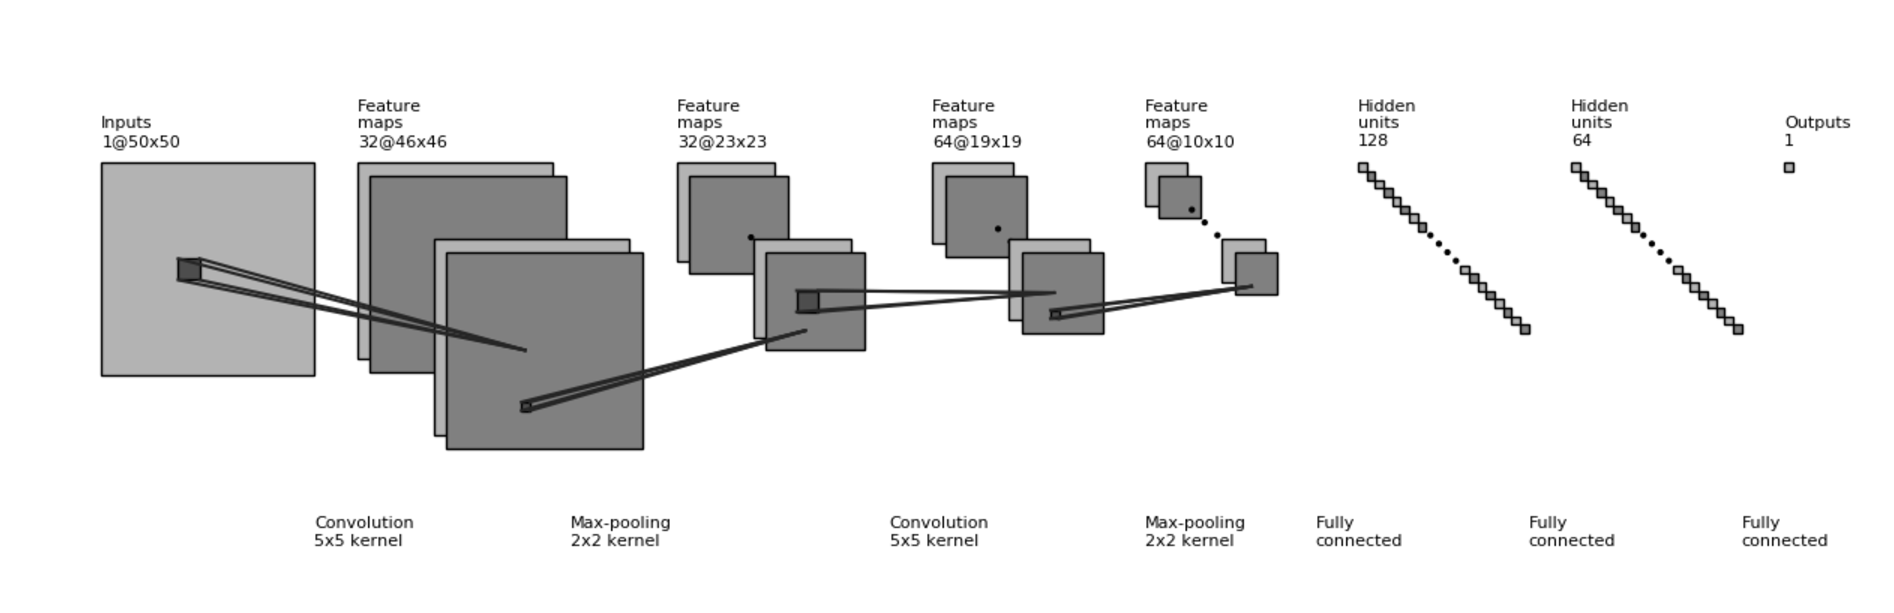
\includegraphics[scale=0.5]{lenet.eps}}
    \caption{LeNet网络结构示意}
    \label{fig:label}
\end{figure}

	\chapter{分析与改进}

\section{过采样vs欠采样}

之前我们使用的是直接拷贝原图片的过采样,这样一共生成了100w万张以上的单词图片,但其中大部分公式图片都是重复的,而且重复度非常高,这样不仅数据多样性低,而且十分容易过拟合,使得在测试集上效果变差。虽然论文图片中大部分都是单词,但单词之间差异远小于公式之间的差异,故我们可以采用欠采样,即在单词图片中随机抽取与公式图片等量的图片。欠采样大大减少了相同程度训练下的数据量,在同等数据量下则大大提高了数据的多样性。虽然导致单词的多样性降低了,但单词的特征本身就比公式特征要简单,故采用欠采样将极大地提高数据的合理性。我们使用欠采样生成了50万左右的单词图片,而使用的原始论文图片则远多于过采样所使用的数量。

\section{网络改进}
\noindent

在参考了AlexNet和VGGNet网络模型之后,结合自己的实际情况,测试时间有限,也没有服务器支持,故自行设计了一个相对简单的网络。网络一共10层,四层卷积层,两层池化层,两层全连接层和一层输出层,此外在最后一个卷积层和第一个全连接层之间加入了一层Spp,前面Spp-Net中也提到了spp层,网络结构如图3.1\footnote{\hbox{This figure is generated by adapting the code from https://github.com/gwding/draw\_convnet}}。
\begin{figure}[ht]
    \centering
    \hbox{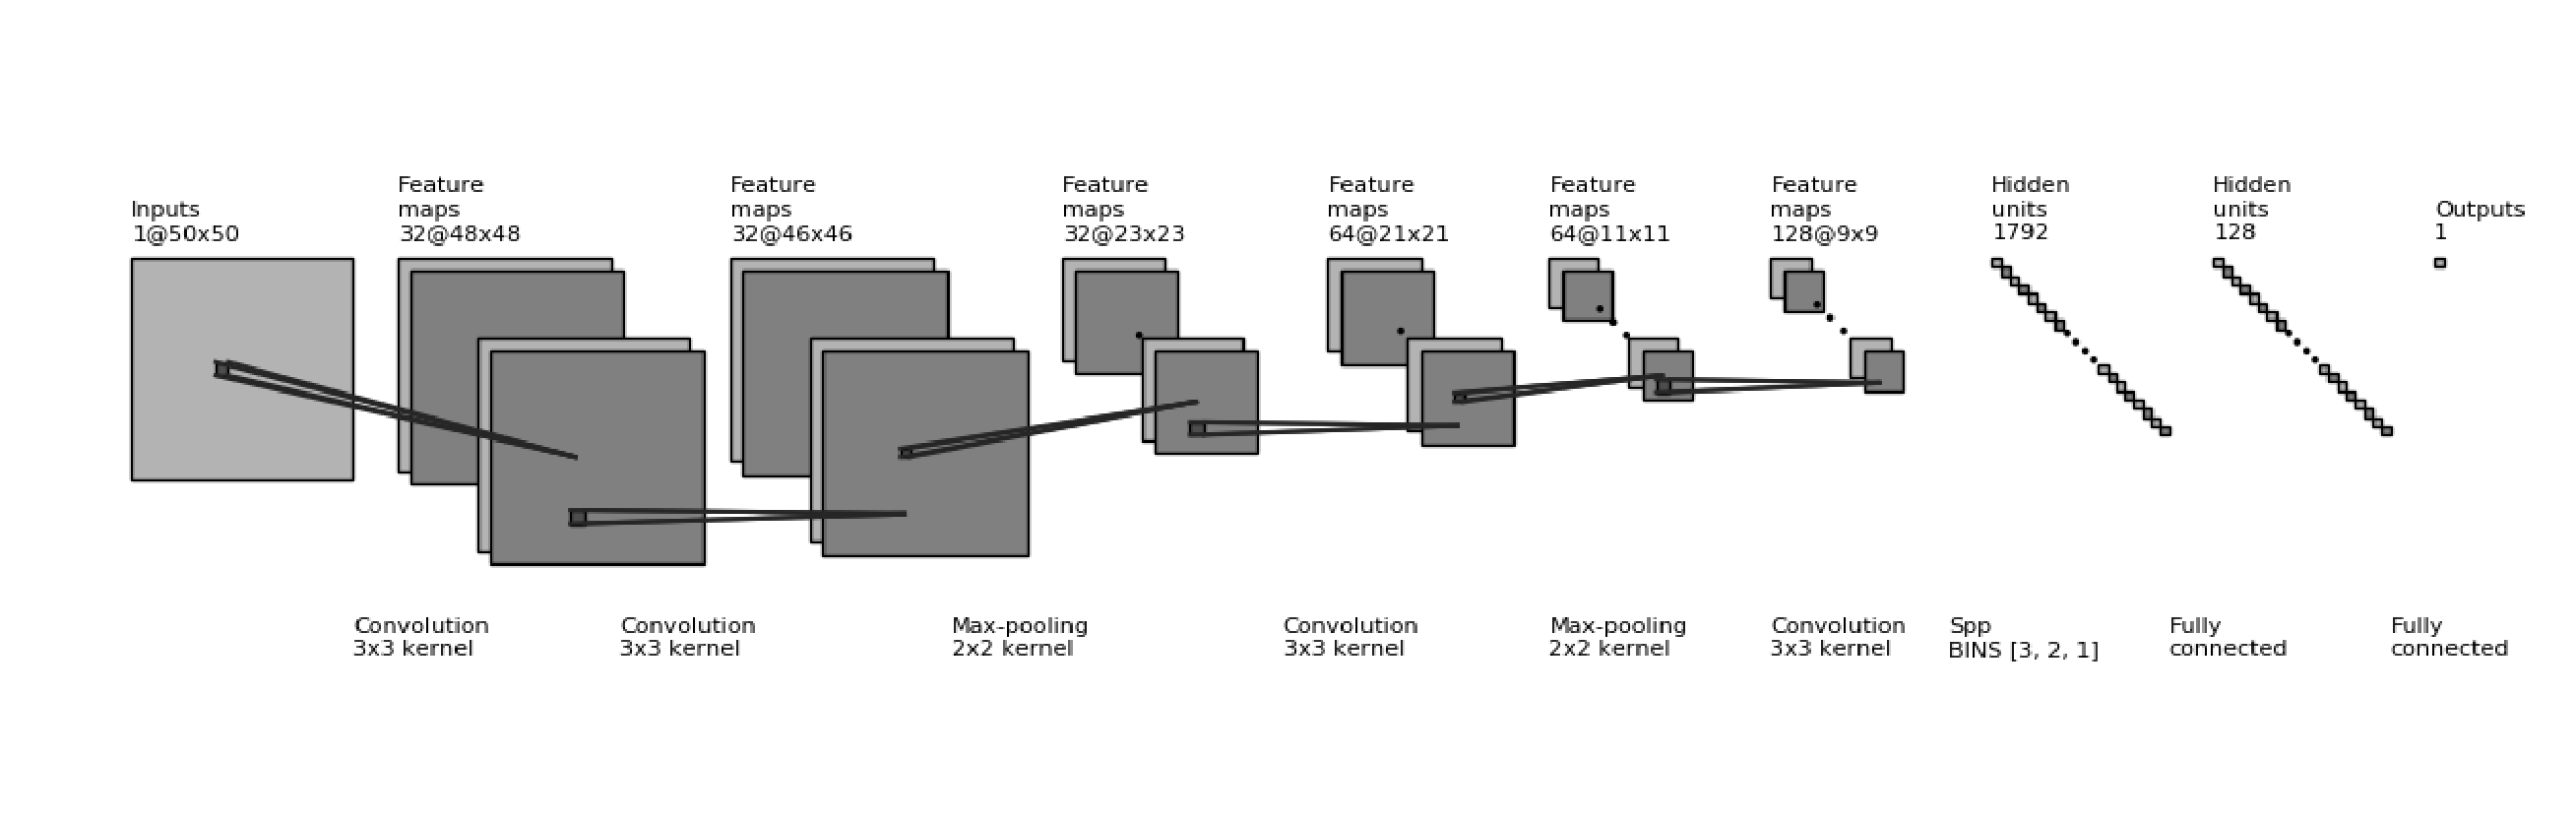
\includegraphics[scale=0.5]{eps/mynet.eps}}
    \caption{我的网络结构示意}
    \label{fig:label}
\end{figure}
spp层是使用了动态尺寸的池化核将任意尺寸的输入池化到固定尺寸的输出。首先需要一个$BINS$来决定输出的尺寸,通常会选择多个输出尺寸来获得更多的信息。如输入图片尺寸为$x \times x$,需要的输出尺寸为$n \times n$,则计算
$$ksize = \lceil \frac x n \rceil$$
$$stride = \lfloor \frac x n \rfloor$$
再利用$ksize$和$stride$做最大池化。对$BINS$中每个输出尺寸都做了最大池化后,把这些数据排成一行输出到全连接层。\cite{spp}最开始是为了实现输入不同尺寸的图片到网络中进行训练所以想使用spp,但由于tensorflow的局限,一是如果输入不同尺寸的图片,就没法使用batch,只能每次输入一个图片;二是spp需要使用图片的动态尺寸,生成动态池化核来进行池化,但tensor自带的池化函数只支持静态池化核,需要自己重写池化函数,又遇到了使用tensor写循环语句的困难。考虑到图片伸缩对本问题的影响不大,故最后改为将输入单词图片都resize到$50 \times 50$,但仍然保留spp层。尽管spp层也需要每次输入的图片尺寸相同,但如果输入图片都变为另外一个尺度,网络也不需要改动,可以直接利用原网络。这样就可以实现多尺度维度的输入来提高效果。

相对于之前的LeNet,网络深度更深,输入图片尺寸的设计也更为灵活,连续使用了两个$3 \times 3$的卷积核来代替原来的一个$5 \times 5$的卷积核则是基于VGGNet的思想。

在损失函数上,考虑到我们的问题中精确度比较重要,故在损失函数中降低了正样本的比重。原本的损失函数为
\[\mathsf{targets} \times -\log(\mathsf{sigmoid}(\mathsf{logits})) + (1 - \mathsf{targets}) \times -\log(1 - \mathsf{sigmoid}(\mathsf{logits}))\]
新的损失函数为
\[\mathsf{targets} \times -\log(\mathsf{sigmoid}(\mathsf{logits})) \times \mathsf{pos\_weight} +(1 - \mathsf{targets}) \times -\log(1 - \mathsf{sigmoid}(\mathsf{logits}))\]
其中$\mathsf{targets}$为数据的标签,正样本为1,负样本为0,我们的数据中公式图片为正样本。$\mathsf{logits}$为网络的输出,经$\mathsf{sigmoid}$后为网络预测的为正样本的概率。$\mathsf{pos\_weight}$则是我们加入的一个比重,用来调节损失函数。当我们令这个比重小于1时,若网络的输入为正样本,则损失函数更小。

\section{CTPN的启发}
\noindent

在独立做完以上工作后,查阅论文时发现在OCR领域的一些文字识别的工作。如CTPN\cite{ctpn}、CRNN等。CRNN主要做的是文字识别工作,而CTPN做的是文字检测。

CTPN做的是自然场景图象中的水平文字检测,主要是在Faster RCNN的基础上结合双向LSTM生成的模型。首先是通过VGG提取特征,将生成的feature map经过一些处理后输入双向LSTM中,生成既包含CNN学习到的空间特征,也包含LSTM学习到的序列特征的特征图。再将特征图通过类似Faster RCNN的RPN网络,获得建议文本位置(text proposals)。CTPN生成的是宽度不变的anchor,通过寻找anchor中心和高度来获得一个小尺寸的建议文本位置,如图3.2,上面是传统的RPN的输出,下面为CTPN输出的建议文本位置,可以看见一个文本有许多小宽度的建议位置,接下来只需要通过文本线构造办法,将这些连接起来形成一个文本检测框。

\begin{figure}[hp]
    \centering
    
\includegraphics[scale=0.5]{eps/rpn.eps}
    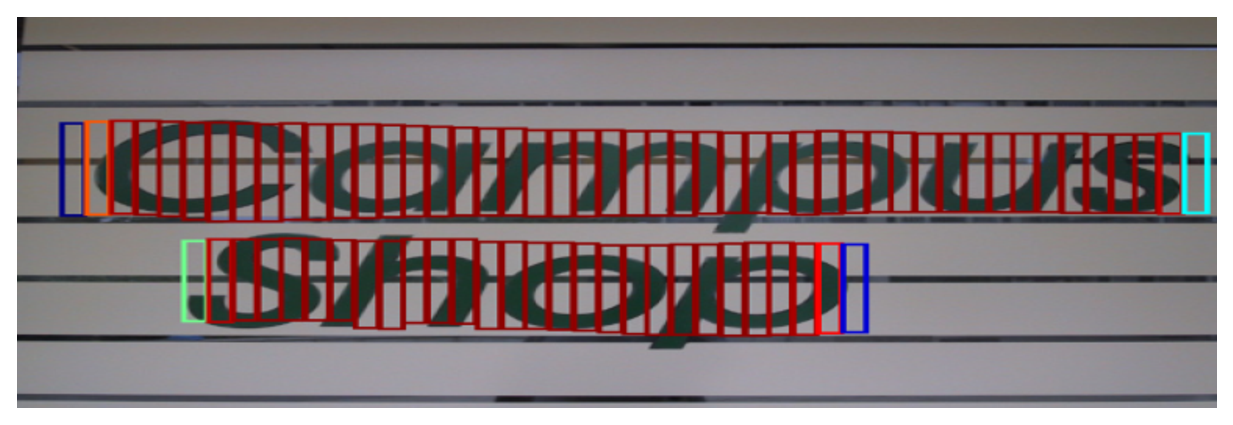
\includegraphics[scale=0.5]{eps/ctpn.eps}
    \caption{CTPN proposals}
    \label{fig:label}
\end{figure}

CTPN的工作是自然场景图象中的文字检测,用在我们的论文图片中有大材小用的样子。但是CTPN的方法给予了我一些启发。在处理单词图片时我们直接将单词图片resize到了固定长宽。单词图片长宽比例很不均匀,若直接resize到方形,原本长宽比例很大的单词和长宽比例接近1的单词就显得不对等,而公式图片的特征变化更为明显。在CTPN中并不直接检测整个文本,而是一段一段地检测文本。故在处理图像时把长宽比大于2的单词分割为两个图片,前者长宽比为1比1,后者为剩下的,递归此操作,最终得到的图片长宽比都不大于2,这样再resize损失的特征大大减少。

\section{更精确的单词切割}

数据预处理将直接影响到最终的结果,特别是文行的切割对结果影响非常大。主要原因是把行间公式和正常文行分开比较困难,而我们的数据中行间公式没有被标记为正类,故测试时网络可能将行间公式预测为正类,而降低precision。在没有进行数据平衡的测试集上,行内公式的数量远小于单词数,而行间公式的数目也不小,而且一个行间公式就会被切割为大量的单词,如果不能很好地排除掉行间公式,尽管网络实际效果很好,precision也不会太高。

首先对于文行单词分割,最大的问题在于没有处理大空白,如果空白数量比较少,则可能单词间空白和字母间空白一起被排除掉,而一行的大空白一般只有一两个,故在处理时只需要将最大的两个空白改为第三的值,然后再进行最小二乘法,就可以比较好地处理这种情况。又由于以上CTPN的启发,单词切割的精确性要求大大降低,只需要位置信息能够还原就足够了。文行分割的问题比较复杂,而且很难做到完全准确的分割。行间公式的情况比较复杂,想简单地通过几个标准把行间公式完全排除比较困难,可以尝试用机器学习去自动学习行间公式的特征从而得到更好的结果,这里只使用了由经验总结出的一些方法。

得到了用空行分割的文行后再继续进行进一步的筛选,需要使用一些指标。之前我们使用的是文行的高度、中心行和、前四分之一行和、开始行和以及结尾行和。中心行和是一个不太好的指标,只采用文行的中心行和来进行判断其准确度比较低,主要是中心行和缺乏代表性,虽然总的来说行间公式的中心行和一般比较小,但如果遇到分数线则会大大增加中心行和,而且中心行和很不稳定,波动的范围比较大。为了解决这个问题首先想的是再中心行附近一定范围内随机取一行来求和来作为标准,这种方法十分不稳定,甚至会导致较大的误差,不能保证结果。最后使用的是文行所有行和的平均,成为平均行和,平均行和比较稳定,区分度也比较好,相应的前四分之一行和也使用平均行和。至于行和高度更是一个极不稳定的指标,尽管有的行间公式高度很大,但有的则与目标文行没有差别,甚至有的目标文行如果含有一些公式符号则比行间公式的高度还要大。因此在筛选时的主要标准是平均行和,高度只作为一个辅助标准。同时为了更精确,求高度的分界线时也使用最小二乘法。平均行和和前四分之一行和相比,后者又具有更好的区分性,因为行间公式开头一段通常是空白,因此主要标准为前四分之一行和,使用平均行和和高度来进行辅助。这样调整之后效果有了很大的改进,但仍然无法完全排除行间公式,故测试结果仍然比实际要差,所以我们将通过直接查看在论文图片上的效果来人工评估一下模型效果。

\section{网络训练结果比对}
\noindent

测试结果评估采用了4个指标,accuracy、precision、recall、F1 Measure。TP为预测正确的正类,FP为预测错误的正类,TN为预测正确的负类,FN为预测错误的负类。accuracy为所有图片预测正确的概率,precision为预测为正类的图片中预测正确的比例,recall为所有正类中被预测正确的比例,F1为precision和recall的调和平均。
\[accuracy = \frac {TP + TN} {TP + FP + TN + FN}\]
\[precision = \frac {TP} {TP + FP}\]
\[recall = \frac {TP} {TP + FN}\]
\[F_1 = \frac {2 TP } {2 TP + FP + FN}\]
为了能够查看在实际图片上的效果,可使用文件formula\_find.py。这个文件将输入的图片先做空白边框去除和单词分割,然后将图片依次传入训练好的网络模型中,得到结果后再使用每张图片的位置信息在原图像上进行标注,对于被分割的公式,在重建时直接将相邻的被预测为公式的单词合并起来,然后用红框标注。

Os使用过采样的数据,训练数据571029张单词图片,测试图片12637张。Us为使用欠采样的数据,训练数据404383张单词图片,测试图片12637张。以上两种没有使用方形单词分割,Sq为使用了方形单词分割作为训练和测试集,训练数据465974张单词图片,测试图片22391张。Us与Sq使用的训练原始数据,即没有经过预处理的数据相同,但方形单词分割会得到更多的图片。Os因为过采样,所以原始数据比后两者要少。

\begin{figure}[hp]
    \centering
    \begin{tabular}{cccc}
    \toprule
    Set& 训练集& 测试集\\
    \midrule
    Os& 571029& 12637\\
    Us& 404383& 12637\\
    Sq& 465974& 22391\\
    \bottomrule
    \end{tabular}
    \caption{各数据集数据量}
\end{figure}

三种模型都以100大小的batch进行5000次训练,结果发现Sq各方面优于Us,Us优于Os。但Os结果实际上已经还不错,故提升的幅度比较小。

\begin{figure}[hp]
\centering
\begin{tabular}{ccccc}
\toprule
Set& accuracy& precision& recall& F1\\
\midrule
Os& 0.9901& 0.9316& 0.9987& 0.9640\\
Us& 0.9904& 0.9343& 0.9975& 0.9648\\
Sq& 0.9946& 0.9418& 0.9995& 0.9698\\
\bottomrule
\end{tabular}
\caption{测试集上结果}
\end{figure}

\section{实际效果演示}
\noindent

三个网络的实际表现都已经非常不错,实际准确率非常高,故接下来主要演示一下结果不准确的部分及其原因。首先是由于文行分割导致的问题,有些过短的行被排除了,如果其包含公式就不会被检测,这样的情况如图。然后是一些公式符号单独成行,但这一行也被排除了,如图。还有有的行间公式没有无法排除掉,造成如图的情况。
\begin{figure}[hp]
    \centering
    \begin{subfigure}[b]{\linewidth}
    \centering
    
\includegraphics[scale=0.3]{eps/a11.eps}
    \caption{\label{fig:fig1}}
    \end{subfigure}

    \begin{subfigure}[b]{\linewidth}
    \centering
    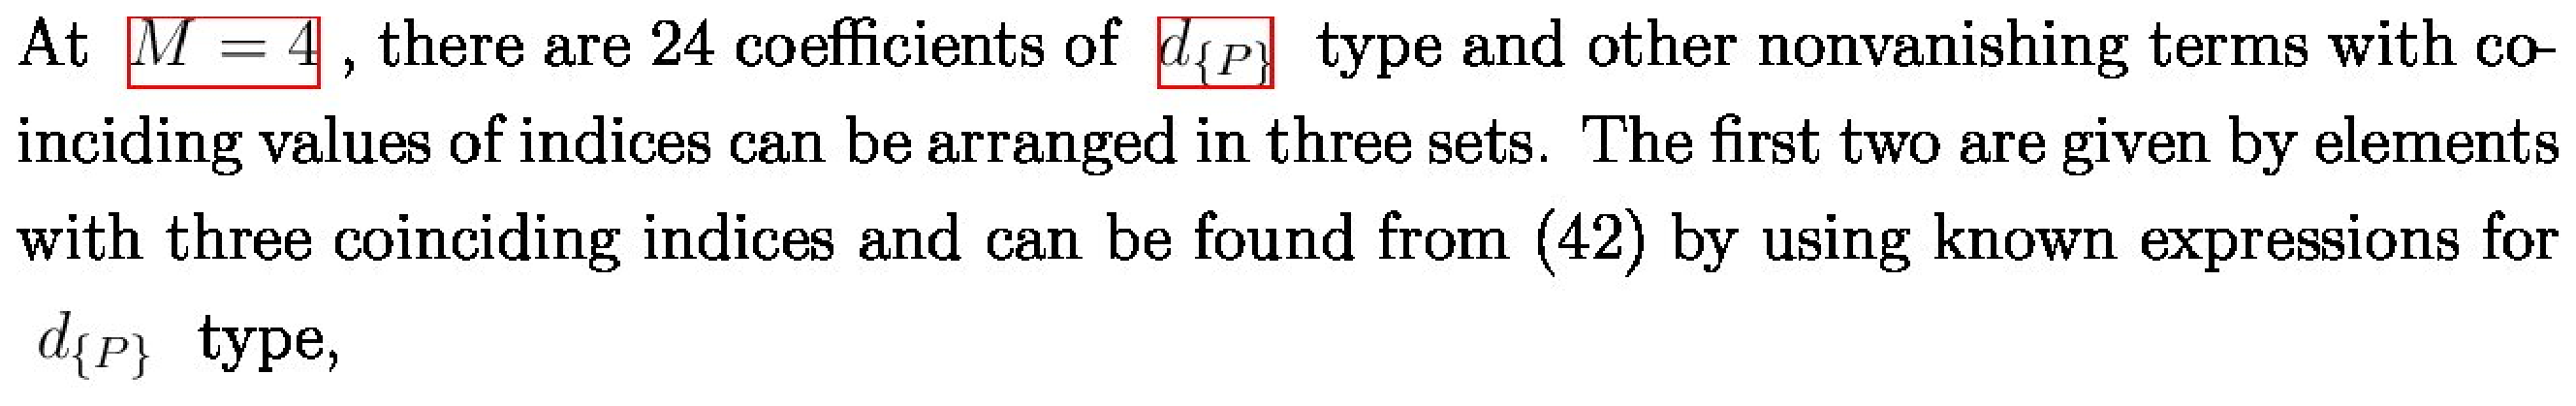
\includegraphics[scale=0.3]{eps/a12.eps}
    \caption{\label{fig:fig2}}
    \end{subfigure}

    \begin{subfigure}[b]{\linewidth}
    \centering   
    
\includegraphics[scale=0.3]{eps/a13.eps}
    \caption{\label{fig:fig3}}
    \end{subfigure}

    \begin{subfigure}[b]{\linewidth}
    \centering 
    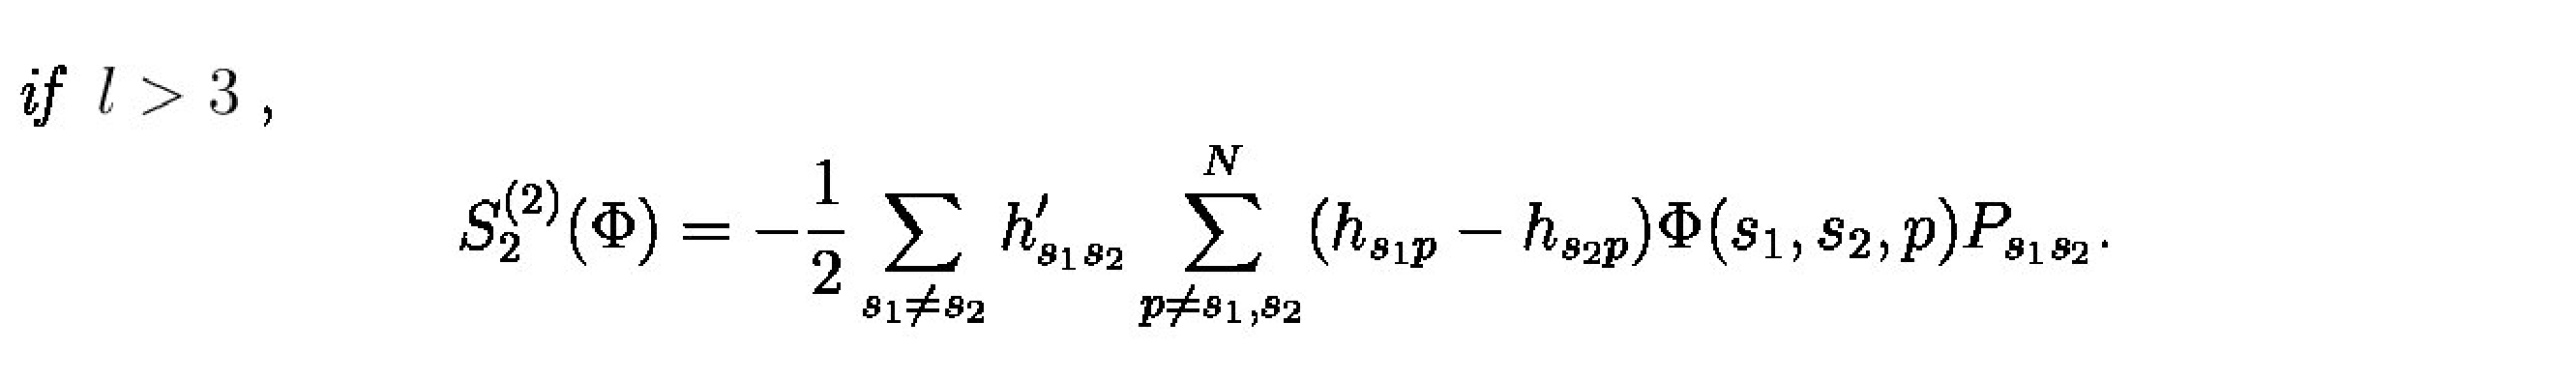
\includegraphics[scale=0.3]{eps/a14.eps}
    \caption{\label{fig:fig4}}
    \end{subfigure}

    \begin{subfigure}[b]{\linewidth}
    \centering 
    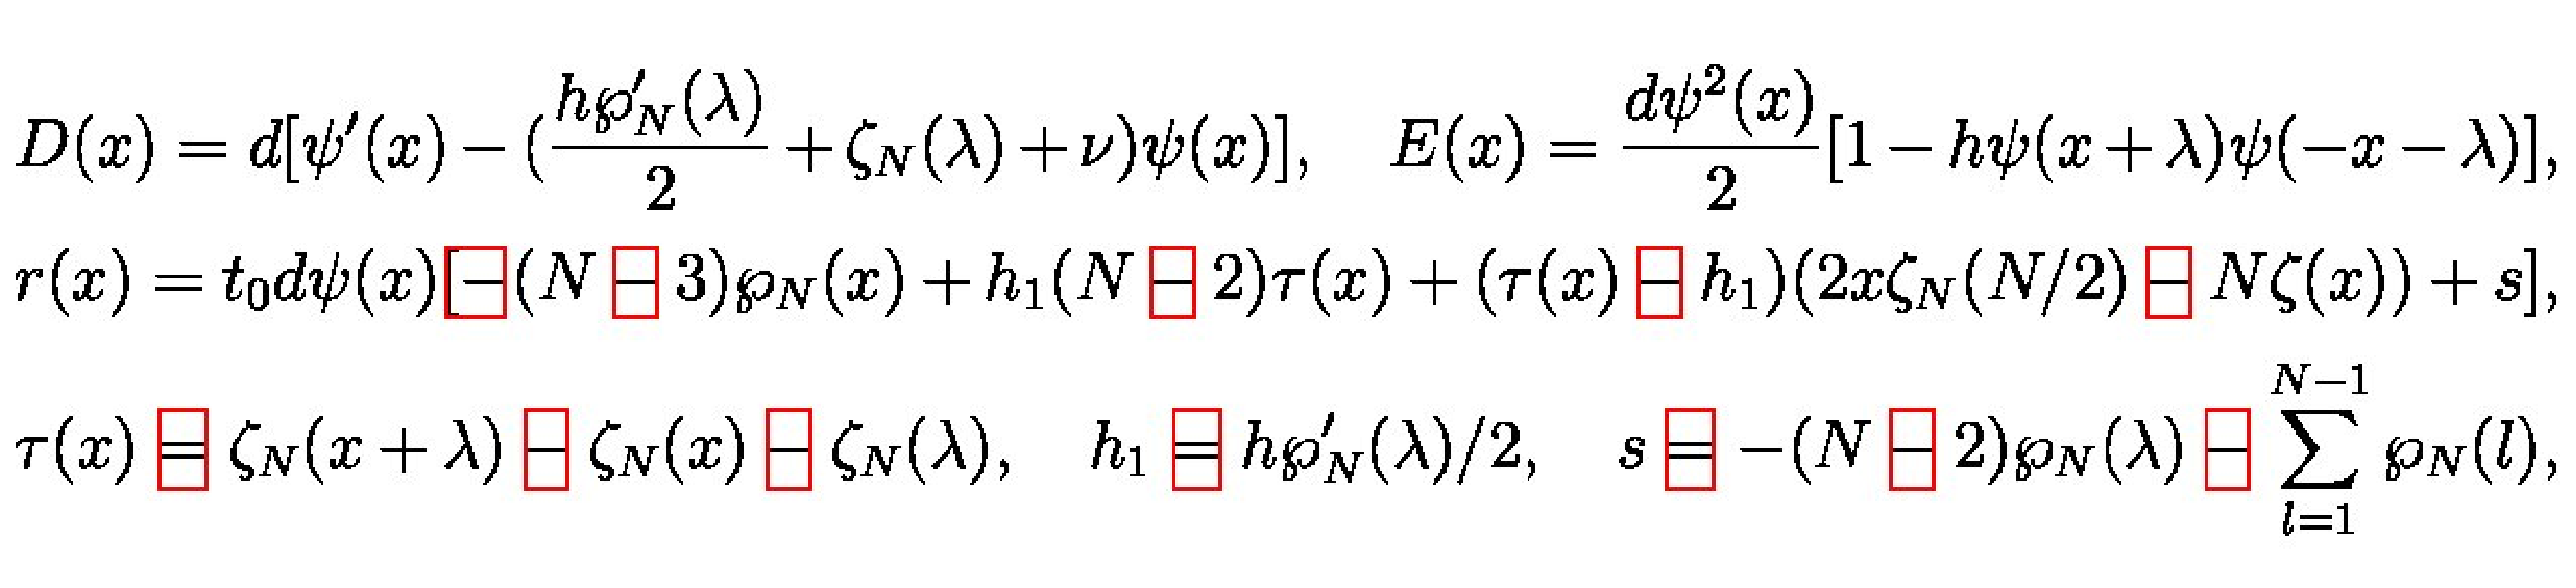
\includegraphics[scale=0.3]{eps/a15.eps}
    \caption{\label{fig:fig5}}
    \end{subfigure}

    \caption{文行分割导致的问题}
    \label{fig:label}
\end{figure}

\begin{figure}[hp]
    \centering
    \begin{subfigure}[b]{\linewidth}
    \centering
    
\includegraphics[scale=0.3]{eps/a21.eps}
    \caption{\label{fig:fig1}}
    \end{subfigure}

    \begin{subfigure}[b]{\linewidth}
    \centering
    
\includegraphics[scale=0.3]{eps/a22.eps}
    \caption{\label{fig:fig2}}
    \end{subfigure}

    \begin{subfigure}[b]{\linewidth}
    \centering
    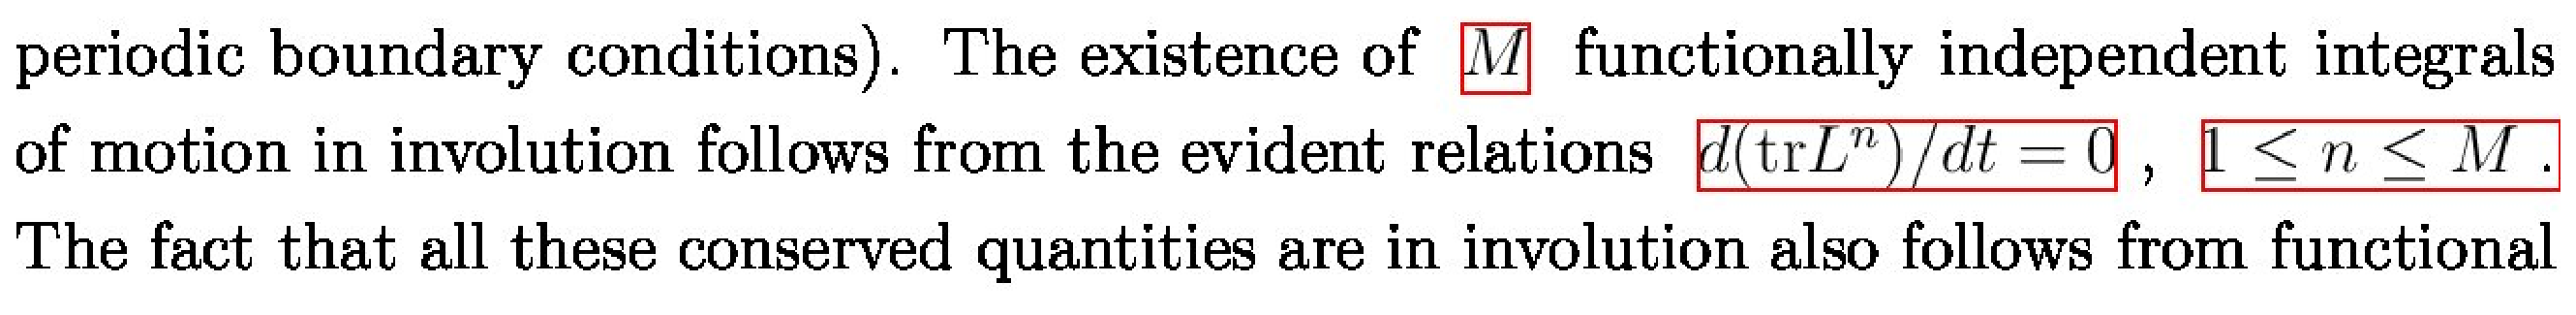
\includegraphics[scale=0.3]{eps/a23.eps}
    \caption{\label{fig:fig2}}
    \end{subfigure}

    \begin{subfigure}[b]{\linewidth}
    \centering
    
\includegraphics[scale=0.3]{eps/a24.eps}
    \caption{\label{fig:fig4}}
    \end{subfigure}

    \caption{网络学习的问题}
    \label{fig:label}
\end{figure}


\begin{figure}[hp]
    \centering

    \begin{subfigure}[b]{\linewidth}
    \centering
    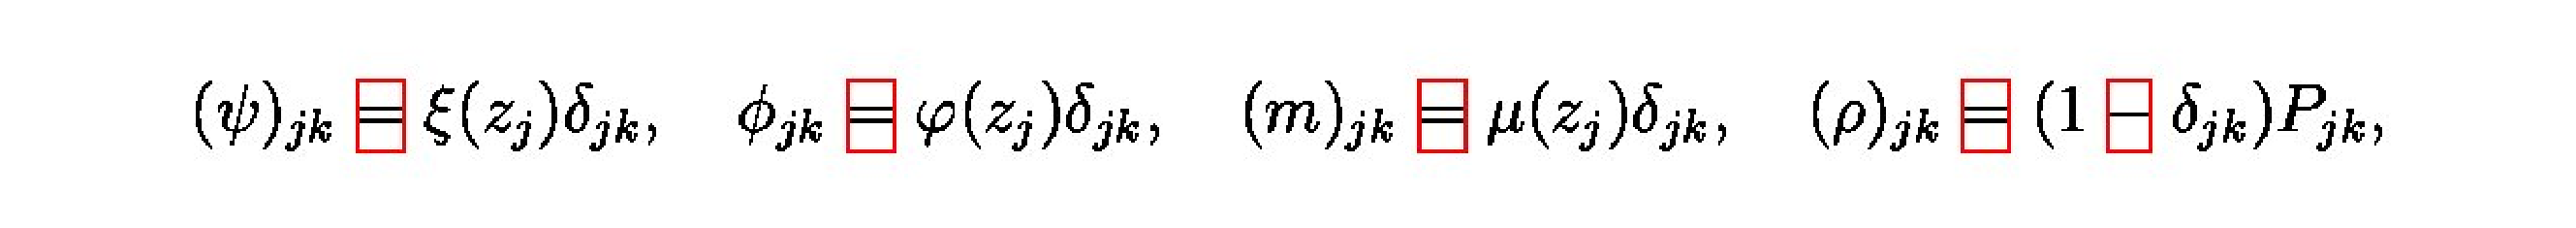
\includegraphics[scale=0.3]{eps/os1.eps}
    \caption{\label{fig:fig1}}
    \end{subfigure}

    \begin{subfigure}[b]{\linewidth}
    \centering
    
\includegraphics[scale=0.3]{eps/os2.eps}
    \caption{\label{fig:fig2}}
    \end{subfigure}


    \caption{Os的问题}
    \label{fig:label}
\end{figure}

\begin{figure}[hp]
    \centering

    \begin{subfigure}[b]{\linewidth}
    \centering
    
\includegraphics[scale=0.3]{eps/us1.eps}
    \caption{\label{fig:fig1}}
    \end{subfigure}

    \begin{subfigure}[b]{\linewidth}
    \centering
    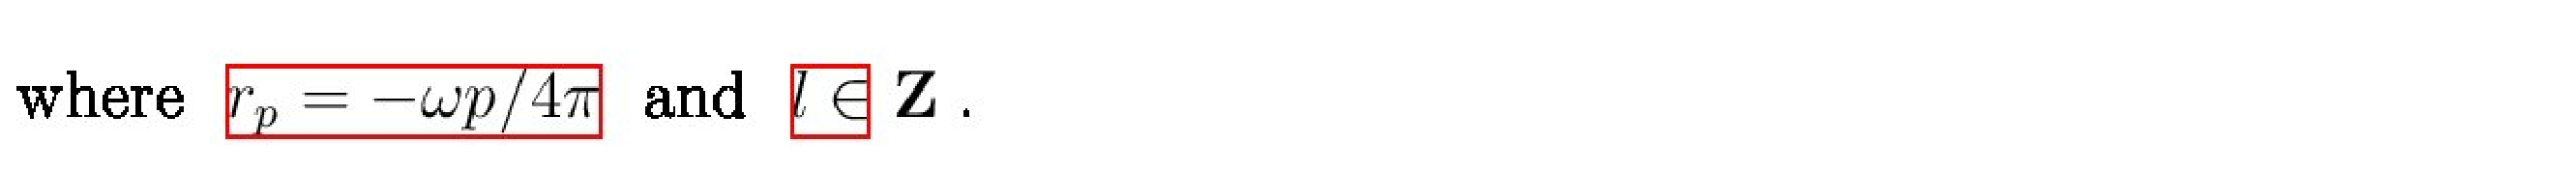
\includegraphics[scale=0.3]{eps/us2.eps}
    \caption{\label{fig:fig2}}
    \end{subfigure}

    \begin{subfigure}[b]{\linewidth}
    \centering
    
\includegraphics[scale=0.3]{eps/us3.eps}
    \caption{\label{fig:fig3}}
    \end{subfigure}


    \caption{Us的问题}
    \label{fig:label}
\end{figure}

\begin{figure}[hp]
    \centering

    \begin{subfigure}[b]{\linewidth}
    \centering
    
\includegraphics[scale=0.3]{eps/sq1.eps}
    \caption{\label{fig:fig1}}
    \end{subfigure}

    \begin{subfigure}[b]{\linewidth}
    \centering
    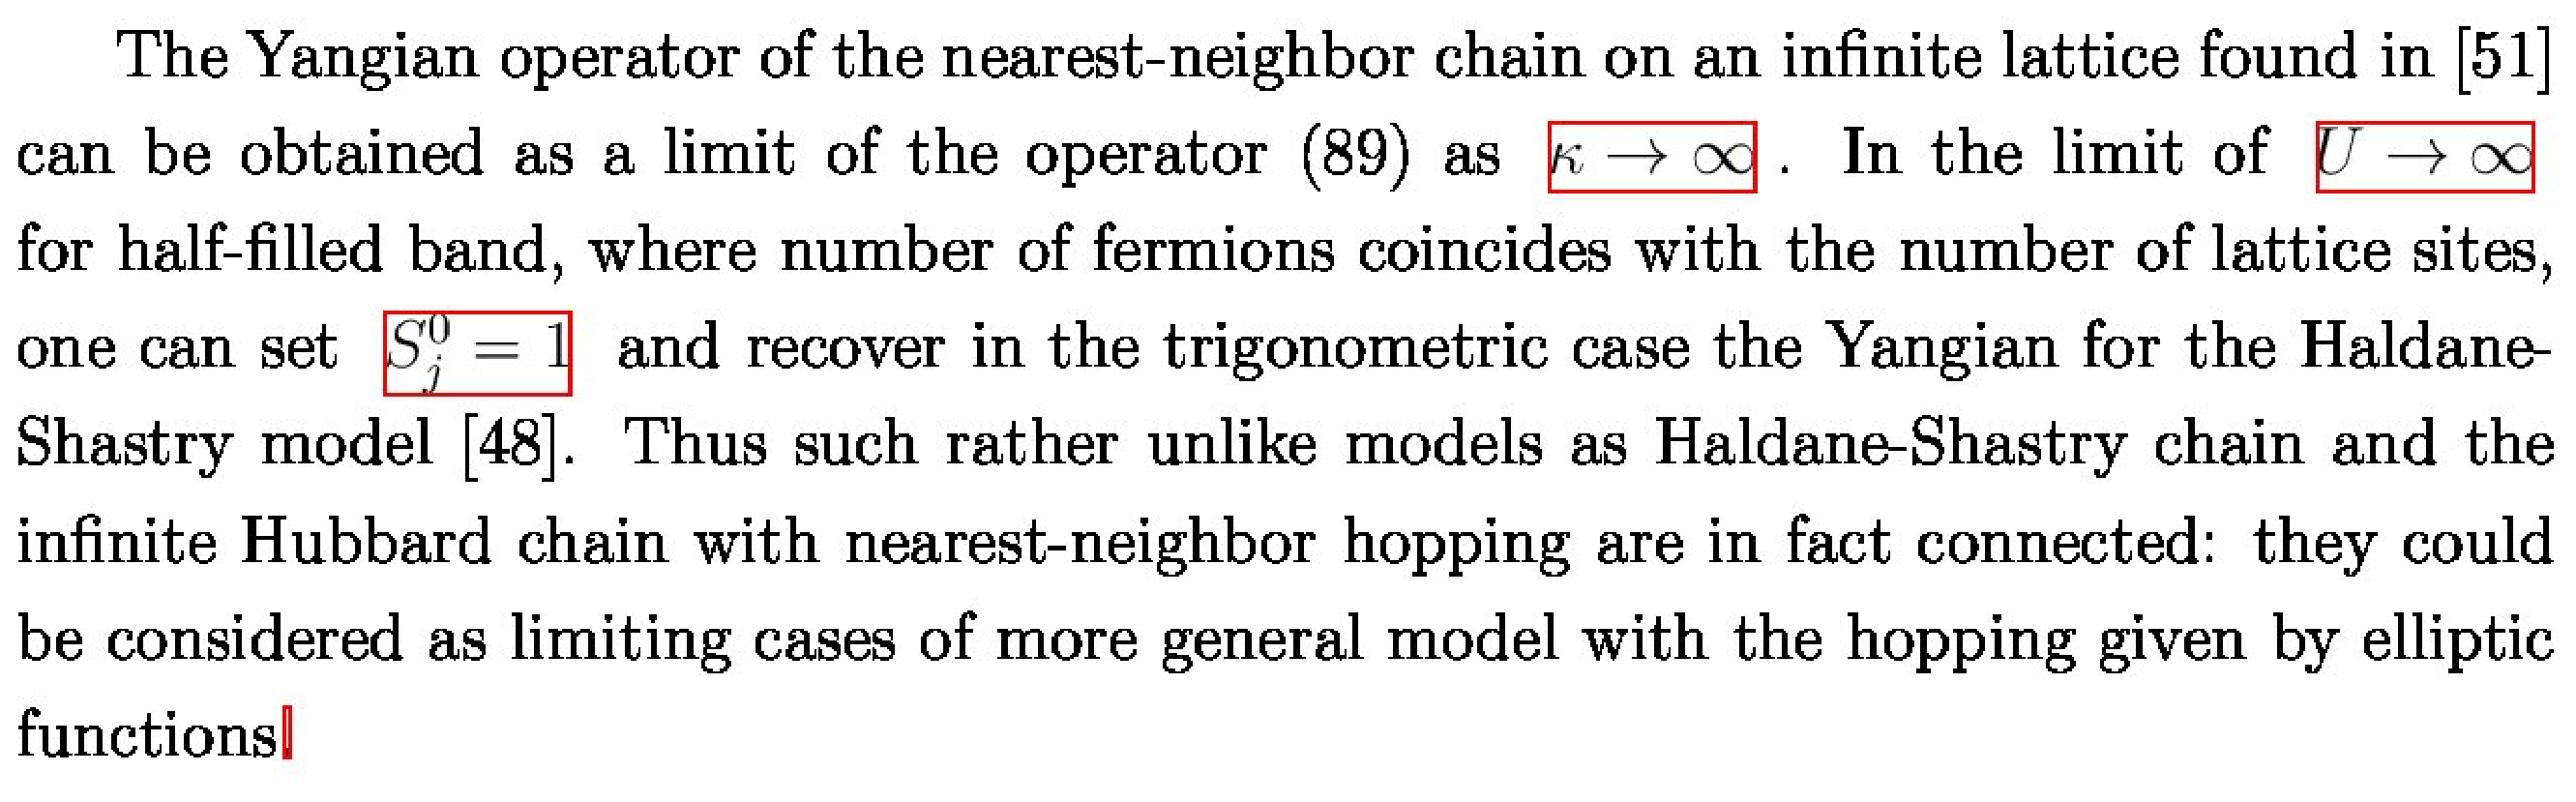
\includegraphics[scale=0.3]{eps/sq2.eps}
    \caption{\label{fig:fig2}}
    \end{subfigure}

    \begin{subfigure}[b]{\linewidth}
    \centering
    
\includegraphics[scale=0.3]{eps/sq3.eps}
    \caption{\label{fig:fig3}}
    \end{subfigure}

    
    \caption{Sq的问题}
    \label{fig:label}
\end{figure}

	% 正文中的附录部分。
	\appendix
	% 排版参考文献列表。bibintoc 选项使“参考文献”出现在目录中;
	% 如果同时要使参考文献列表参与章节编号,可将“bibintoc”改为“bibnumbered”。
	\printbibliography[heading = bibintoc]
	% 各附录。
	\include{chap/encl1}

	% 以下为正文之后的部分,默认不进行章节编号。
	\backmatter
\end{document}

% vim:ts=4:sw=4
